%\documentclass{sig-alternate-10pt}
\documentclass[letterpaper,twocolumn,11pt]{article}
\usepackage{url}
%\usepackage{usenix,epsfig,endnotes}
%\usepackage{fullpage} 
%\setlength{\textwidth}{6.75in}
%\setlength{\oddsidemargin}{-.125in}
\usepackage{graphicx}

\usepackage{natbib}
%\usepackage{subfigure}
%\usepackage{ifpdf}
%\usepackage{multicol}
%\usepackage{amsmath, amssymb, amsthm}
%\usepackage{rotating}
%\onehalfspacing
%\newcommand{\tbd}[1]{[{\bf{#1}}]}

\newcommand{\projectname}[1]{PCC}
\newcommand{\tbd}[1]{}
\newcommand{\ie}{{\it i.e.}}
\newcommand{\eg}{{\it e.g.}}
\newcommand{\etc}{{\it etc.}}
\newcommand{\apriori}{{\it a priori}}
\newcommand{\eat}[1]{}

\usepackage[usenames,dvipsnames]{color}
\newcommand{\justine}[1]{{\color{ForestGreen}\bf JS: {#1}}}
\newcommand{\andi}[1]{{\color{blue}\bf AW: {#1}}}
\newcommand{\colin}[1]{{\color{Red}\bf CS: {#1}}}
\newcommand{\scott}[1]{{\color{Purple}\bf SS: {#1}}}

\setlength{\columnsep}{.25in}
\setlength\topmargin{-.5in}
\setlength\textheight{8.5in}
%\usepackage{verbatim}
%\usepackage[compact]{titlesec}
%\usepackage[small]{caption}
\usepackage{times}

% Squeeze out the whitespace!
%\setlength{\parskip}{0pt}
%\setlength{\parsep}{0pt}
%\setlength{\headsep}{0pt}
%\setlength{\topskip}{0pt}
%\setlength{\topmargin}{0pt}
%\setlength{\topsep}{0pt}
%\setlength{\partopsep}{0pt}
%\usepackage[compact]{titlesec}
%\titlespacing{\section}{.5pt}{*.2}{*.2}
%\titlespacing{\subsection}{.5pt}{*.2}{*.2}
%\titlespacing{\subsubsection}{.5pt}{*.2}{*.2}


\title{\vspace{-40pt}\projectname{}: Cross-Layer Debugging for the \\ Software-Defined Networking Stack}

%\author{Colin Scott and Andreas Wundsam and Justine Sherry and Scott Shenker}
\author{Paper \#n}

%        \begin{multicols}{2}{{\it Draft - Please do not distribute.}}\\
%\author{Paper \#69, 14 Pages}

\date{}
\begin{document}
    \maketitle

\abstract{
{\it
Software bugs are inevitable in software-defined networking (SDN) control planes,
and troubleshooting
is a tedious, time-consuming task.
In this paper we discuss how one might improve
control software troubleshooting by presenting a technique
for automatically identifying
a minimal sequence of inputs responsible for triggering a given bug.
We present three preliminary case studies of real bugs we have found in open source SDN control
platforms---Floodlight, POX, and NOX---and
illustrate how the minimal sequences our technique found were useful for
understanding the root cause of the bugs.

\vspace{45pt}
}

\section{Introduction}
\label{sec:intro}
The SDN platform's $raison\text{ }d'\hat{e}tre$ is to 
hide complexity from control applications. To this end, modern platforms perform
replication, resource arbitration, failure recovery, and network 
virtualization on the control application's behalf. 

While these measures are effective in simplifying control applications,
they do not remove any complexity from the overall system. Rather, they merely move the complexity
from control applications into the underlying SDN platform.

As in any software system, additional complexity increases the probability of
bugs. And unfortunately for the network operator, finding bugs in the platform requires
access to precisely the details hidden from the control application.
When operators encounters erratic behavior in their network, the error's root
cause may lie in their own policy specification, or in the SDN platform
itself. To deal with the latter case, they must trace through
multiple layers of abstraction: virtualization logic, distribution logic, and
network devices.

As it stands, the SDN platform provides meager support for troubleshooting.
The predominant troubleshooting method is log analysis: manually
specifying log statements at relevant points throughout the system,
collecting; gathering; and ordering distributed log files; and analyzing the
results {\it post-hoc} when a error is encountered in production. Besides its
apparent tediousness, this approach is lacking in several ways: logs events
are enormous in number, impossible to aggregate into a single serial
execution of the system, and often at the wrong level of granularity to be of
use.

Recent work has contributed much-needed improvements to the highest (control
application) and lowest (dataplane forwarding tables) levels of abstraction, 
but no principled troubleshooting mechanism exists yet for the SDN platform.
NICE applies concolic execution and model checking to SDN control
applications, thereby automating the testing process and catching bugs before
they are deployed~\cite{nice}. Aneater~\cite{anteater} and HSA~\cite{hsa}
introduce mechanisms for checking static invariants in the dataplane.

It would be unthinkable to introduce a new programming language without a
debugger. Similarly, we think it highly undesirable to deploy SDN-based
networking without a viable troubleshooting paradigm. 

Correctness of the SDN platform can be stated concisely: high-level policies
should correspond with low-level configuration. We observe that the structure
of the SDN platform, graphs at every layer, enables a straightforward
algorithm to check this invariant. Our algorithm, which we term correspondence checking,
enumerates all inconsistencies at any point in time and isolates the
root cause of an inconsistency to a particular component of the system.

In eventually-consistent systems such as software-defined
networks however, transient inconsistencies between network policy and actual network
behavior are an inevitable state-of-affairs.
In such an environment, it does not suffice for troubleshooting tools to
simply enumerate inconsistencies; they should also aid the developer
in identifying which are related to serious problems, and which are
harmlessly ephemeral. To this end we present \simulator.
\Simulator allows troubleshooters 
to sift out pernicious inconsistencies by tracking the life cycle of problems 
both forward and backward in time.

We have implemented prototypes
of correspondence checking and \simulator. Our code is publicly available
at~\cite{github}.

The rest of this paper is organized as follows. In \S\ref{sec:overview},
we present an overview of the SDN stack and its failure modes.
In \S\ref{sec:approach} we present correspondence checking and
\simulator in detail. In \S\ref{sec:evaluation} we present
two use-cases and a preliminary performance evaluation
Finally, in \S\ref{sec:related_work} we discuss related work,
and in \S\ref{sec:conclusion} we conclude.


\section{SDN Overview}
\label{sec:overview}
In this section we review some of the key aspects of SDN systems, starting with the nature of the control plane and then the process of troubleshooting.

\subsection{SDN Control Planes}
Network operating systems, which are the key component of the SDN software
infrastructure, consist of controller software running on a replicated set of
servers, each running a controller instance. The replicas typically use a
consensus protocol for leader election and a distributed database to ensure
consistency of state~\cite{onix}. A controller receives input events and
statistics from switches (whether physical or virtual), configuration and
policy changes via a management interface, and sometimes packets from the data
plane. In response to one or more of these events, the
controller issues packet forwarding instructions to the switches.  All input
and output events are asynchronous, and individual controllers may fail at any
time. These controller instances may communicate
with each other over the network they manage, or use a separate dedicated
network. In either case, the controllers may become partitioned.

\subsection{Bugs, QA Testing, and Troubleshooting}
The goal of a network control plane is to configure the switch forwarding entries so as to
enforce one or more invariants, such as connectivity (\ie, ensuring that a
routing path exists between every endpoint pair), isolation and access control (\ie, various limitations on
connectivity), and virtualization (\ie, ensuring that packets are handled by
the network's switches in a manner consistent with what would happen in the specified virtual
network). A bug causes an invariant to be violated. Bugs can occur in the
configuration management system, \eg~OpenStack~\cite{quantum} (\ie, the
management system or a human improperly specified their goals), or it
can occur within the SDN control plane. In this paper we focus on bugs in the
SDN control plane after it has been given a configuration from the management
system, largely because the goal of SDN is to simplify the network management
system and push complexity into the control plane.

In commercial SDN development, software developers work with a team of QA engineers whose
job it is to find bugs.  The QA engineers run test scenarios that involve
sequences of external events such as failures, migrations, or policy changes
on large network testbeds, either real or emulated.
If they detect an invariant violation, they hand the resulting trace to a developer for analysis.

The space of possible bugs is enormous, and it is often difficult and time
consuming to link the
symptom of a bug (\eg, a routing loop) to the sequence of events in the QA
trace (which includes both the external events and monitoring data on the
system itself), since QA traces often contain a wealth
of extraneous input events, all of which may appear characteristic of normal
operating conditions at first glance. Consider that an hour long QA fuzz test, assuming 8.5 network error events per
minute~\cite{Greenberg:2009:VSF:1592568.1592576} and 500 VM migrations per
hour~\cite{Soundararajan:2010:CBS:1899928.1899941},
would contain $8.5 \cdot 60 + 500 \approx 1000$ inputs.

The act of {\em troubleshooting} involves identifying which sequence of external events is most directly responsible for triggering the bug; identifying these events helps the developer understand which code paths might hold the offending code. Currently, painstaking manual analysis of logs is the {\em de facto} method of troubleshooting distributed systems in practice.
{\em Debugging} is then the act of tracking down the error in the code itself,
given a sequence
of triggering inputs. The smaller the sequence of triggering inputs, the easier debugging will
be. Minimizing the sequence of triggering inputs is the goal of our system.



\section{Architecture}
\label{sec:architecture}

% Research question here?
% Going to be challenging to have this not come across as a software design
% spec.. Let's try to get this section over with as little text wasted as
% possible... I feel silly writing these sections, since I ALWAYS skip over
% them when I'm reading other people's papers...
\projectname{} is our realization of correspondence checking and \simulator{}
as a useful platform to troubleshoot SDN controllers. In this section we discuss
our goals in designing \simulator{}, and the challenges we encountered in the process
of realizing these goals.

\subsection{Design Goals: The 7 rules of \projectname{}}

We seek to build a system that facilitates the process of troubleshooting.
First and foremost, we hope that \projectname{} can reproduce difficult bugs
observed in production networks, and automate the process of diagnosing their
causes. We also envision \projectname{} being used as a common repository for difficult, corner-case
scenarios known to have caused problems for other control platforms in the past.
Given these potential use cases, we require the design of the system to be
driven by the following requirements:

\noindent{\bf (1) Realistic Network Sizes.} We focus on large, production SDN
deployments. As today's datacenters may contain up to 100,000 hosts and 10,000
switches, our simulation infrastructure must be able to support large numbers
of switches.

\noindent \textbf{(2) Control plane focus} We expect the dynamism in our system to stem from
\emph{control plane events}. Typical rates of control plane events must thus be
handled, and control plane events must be modeled precisely. Conversely, we
don't expect to handle a realistic amount of dataplane traffic, which is
intractable for a software solution, and largely irrelevant in current networks (because they are mostly proactive, so control planes are not being driven by packet arrivals).

\noindent \textbf{(3) Controller choice} Our system should run with existing production
controllers with minimum additional instrumentation. To allow for wider adoption, we don't want to limit ourselves to
a particular controller implementation.

\noindent \textbf{(4) Full determinism} We want our simulation environment to be fully
deterministic, such that repeated simulations with identical initialization values
yield provably identical results. This creates a challenge in conjunction with our goal (3).

\noindent{\bf (5) Comprehensive Failure Modes.} \projectname{} should
support a wide range of failure modes at all components in the
system, including switch and link failures and message drops, delays and reorderings.

\noindent\textbf{(6) Corner cases investigation} The potential state-space in a large-scale network
is intractably large \colin{Reviewer OD: do a better job of describing the
relationship of our work to model checking}.  We focus on interesting cases, as recorded, e.g., in production, or
found through interactive evaluation. To investigate related error conditions,
we \emph{fuzz} the input traces.

\noindent\textbf{(7) Interactivity} The system should be fast enough for interactive exploration through
an operator.

\medskip

While none of these requirements were particularly difficult in isolation, taken in aggregate they posed some difficulties, as we now recount.

\subsection{Components}

As depicted in Figure \ref{fig:system}, \projectname{} combines several
components to facilitate the process of troubleshooting SDN platforms:
\projectname{} takes input
from production traces, interactive manipulation, and synthetic trace
generation, and fuzzes these inputs to ensure that fixes are sufficiently general;
\projectname{}'s simulator supports large, sophisticated networks;
\projectname{} provides a deterministic, code-agnostic execution environment
for running SDN control software; and provides efficient algorithms for
checking correspondence throughout the system execution. We now provide an
overview of each of these components, and the challenges we encountered in
realizing our goals.

\begin{figure*}[!t]
  \centering
  \includegraphics[width=0.8\textwidth{}]{../diagrams/architecture/architecture.pdf}
  \caption{System architecture. \colin{Andi: can haz new diagram? :P}}
  \label{fig:system}
\end{figure*}

\noindent{\bf Trace Input And Fuzzing.} Since a major goal of \projectname{} was
to support a wide range of usage scenarios, % WAT does that even mean
we provide support for three different methods for generating network trace
inputs. The most common method is to insert failure and topology change logs
from production deployments into the simulator for replay. Input traces may
also be produced synthetically with configurable, random probabilities for
network events. Lastly, we support interactive use, where the troubleshooter
has complete control over network events, and is thereby free to explore her
intuitions in order to reproduce a failure mode she has in mind.

\noindent{\bf Simulator.} We have built a simulator for SDN networks,
where network devices and hosts are modeled as lightweight python objects.
\colin{Reviewer OA: python objects creep in to the writing} Within a single thread, we
are able to deterministically model the execution of very large networks.
Our simulated model supports a wide
range of failure modes, and provides fine-grained control over event
orderings, component failures, and other aspects of the system execution. Our
simulator currently supports switch failures, link failures, arbitrary packet
re-orderings, drops and delays, and a fully general control plane.

The main challenge we encountered in the design of the simulator was
maintaining large numbers of TCP connections to the
controller(s). Although the controllers themselves may be spread
over multiple physical servers, the main simulator must nonetheless handle all
TCP connections between switches and controllers within a single process.
We ultimately ended up using epoll to avoid limitations of the UNIX select
implementation.

\noindent{\bf Controller Sandbox.} One of our major goals for \projectname{}
was to be able to run any SDN controller on top of the platform, with minimal
code changes to the controllers themselves. In addition, control servers
running on top of the simulated network must support deterministic execution
for reproducible results.

Currently we run applications as UNIX processes outside of the simulator.
We note however that there are a number of approaches for achieving deterministic
replay for external software. For example: a software determinism layer (e.g.
deterministic random number generators \colin{Reviewer OA: Whenever I see
replay, I worry about dealing with nondeterminism and pseudorandom number
generators. It was not clear how you are dealing with these issues.}) is
extremely lightweight, but requires modifications to the external software;
binary rewriting does not require any modification to the external
software's source code, but incurs moderate performance overhead; and VMs
fully support deterministic replay, but only a relatively small number of VMs can be run
on a single machine. We hope to leverage this previous work in future versions
of \projectname{}. Nonetheless, our architecture does not prevent us from
running controllers on different physical
servers in case we encounter memory or CPU bottlenecks.

\noindent{\bf Correspondence Checking.}
\projectname{} leverages the hassell library provided by HSA~\cite{hsa}
to implement the correspondence checking algorithm. We optimize the code
slightly to run efficiently on large networks; in particular, we parallelize
symbolic packet propagation to a large number of subtasks. Correspondence
checking currently requires a small code change to the controller to fetch
the platform's view of the network state.

\projectname{} is written in roughly 5,000 lines of python, and is publicly
available. [anon]


\section{Evaluation}
\label{sec:evaluation}
% Just realized: b/c of anonymity, the PC can't chastise us for 
% running our system on our own code -- we can't tell them that it's our code!
We applied \projectname{} to three SDN control platforms: 
Frenetic, POX, and Floodlight. We found 1 bug for each platform.
The bug in Frenetic demonstrates 
the utility of checking correspondence between high-level policies and
low-level configuration (without needing to specify invariants). The bugs in 
POX and Floodlight demonstrate the importance of the simulator's ability to 
programaticaly prioritize persistent policy-violations and infer their minimal
causal sets. In addition to describing bugs, we show that \projectname{} is able 
to simulate and check large networks quickly.

\subsection{Case studies}

% Outline for bug reports:
%  - Describe each system under test
%  - Describe bugs found
%  - Lessons learned from finding bugs
\colin{New structure: describe each system under test, describe bugs found,
described lessons learned from finding bugs. First Frenetic, which is
relatively trivial. Then POX, which is our own code, but demonstrates in a
really nice fashion what the simulator sees, and how that's easier to
understand than the status quo. And
lastly, the Floodlight case which is really awesome.}
Here we present a hypothetical use-case from two perspectives
for correspondence checking and \simulator{}.

\noindent{\bf Network Operator.} An enterprise network
operator pays a third-party SDN provider to virtualize their network
and run it in the cloud. The network operator receives a complaint
from an internal team that two servers cannot reach other, and 
verifies the reachablility problem with {\tt ping}. Unsure
whether the problem is in her ACL/routing rules 
or in the underlying SDN platform, the
operator runs correspondence checking on a snapshot of the network state. She
finds that there is an inconsistency between her policy and the network state, 
and proceeds to call up the third-party SDN provider to complain
about the problem.

\noindent{\bf SDN Developer.} A developer at the third-party SDN
company receives the customer's trouble-ticket and begins to investigate the
problem. The developer examines the system logs and sees a
long list of link status events, control server reboots, VM migration events,
and other diagnostic information. These events are numerous (the
datacenter contains 8,000 switches and more than 100,000 hosts) and
interleaved, so the developer is unsure what caused the problem.
The developer feeds a snapshot of the network from before the
trouble-ticket was issued into the simulator, and
begins replaying the execution of the system. The developer runs
correspondence checking and finds a substantial list of policy-violations,
manifesting as loops, blackholes, and other problems.
The developer excludes all external events
unrelated to the two disconnected hosts. As the developer is stepping through the execution, he periodically
runs correspondence checking and tracks the policy-violations over time. He
finds that most violations resolve within a short time. However, he
eventually encounters a blackhole that lasts a considerable time. The
developer backs up the execution to the point when the blackhole begins, and
observes a switch failure followed directly by a reboot of the switch's parent
controller. A correspondence check between the intermediate layers of the SDN
stack indicate that the problem is present in the
physical view, but is not manifest in the virtualization layer. The developer adds log statements to the platform's failover
logic, and re-runs the execution. The developer eventually verifies that the
controller pushed a routing change to the failed switch's neighbors, but did
not update the platform's representation of the network state. Upon closer
examination, the developer finds that the new parent controller for that
portion of the network assumed that the platform's
representation of network state was up-to-date. As such, the partially installed flow entries remained
in the neighboring switches, resulting in the blackhole. The developer fixes
the platform's recovery code, adds this case to the platform's integration
test suite, and pushes the change to production. 

\subsection{Distributed controller failover race condition}

More complex bugs and race conditions occur when controllers need to be
distributed and fail-over mechanisms between the individual instances are
required for fault tolerance. Consider the following case described in the
Floodlight~\cite{floodlight} source code\footnote{Note this issue was
independently discovered}: For high availability, floodlight can run as a
distributed controller, with switches connecting to several controllers at the
same time. In this setup, one controller assumes the role of \emph{master} and
thereby gains the authority to issue state changing requests to the switches.
The other controllers are in \emph{slave} mode and thus do not perform any
state-changes on the switch. Here, a race condition can occur when a switch
connects to the controllers shortly after the master controller has died, but
before a new master has been selected. In this case, all controllers will be in
the slave role and thus will not take responsibility for clearing the switch
flow table. At some point, one of the controllers is elevated to to
\emph{master} role and will proceed to manage the newly connected switch, based
on an inconsistent flow table.

Using \projectname, we were able to reproduce the problem. To this end, the
emulated switches in the simulator support the \emph{role} vendor extension to
connect to several controllers. The inter-controller synchronization and heartbeat
protocol is proxied through the simulator for control over the timing. After the
master controller dies, a new switch is associated with the slave controllers, and
integrated into the system with an unmerged flow-table, resulting in a persistent
inconsistency between the flow-table in the controller and the switch.

\subsection{Overhead}

\noindent{\bf Record and Replay Overhead.} In contrast to general record-and-replay
mechanisms, the amount of recorded state needed for
high-fidelity replay is tractable. With proactive flow installation, 
updates are pushed to routing tables over a relatively long time scale; periodic
FIB snapshots along with a log of link state events, control server
downtime, and host mobility information suffice for our purposes. As a point of reference, the Cisco 7000 
core switch model supports a maximum of 128K MAC entries and
128K ACL entries~\cite{cisco7000}. Assuming 36 bytes per flow entry,
(larger than the OpenFlow 13-tuple), each FIB will contain a maximum of 9216
bytes, uncompressed. A datacenter of 100,000
hosts includes roughly 8,000
switches~\cite{Al-Fares:2008:SCD:1402958.1402967}.
Therefore a snapshot of the FIBs of the entire network takes up roughly 74 MB.
The VL2 paper reports 36M network error events over one year over 8
datacenters, which implies 8.5 error events per minute per
datacenter~\cite{Greenberg:2009:VSF:1592568.1592576}.
Suppose we took a snapshot of the FIBs in the network every second. 
Then we would need to store roughly 4GB, uncompressed, per minute, a relatively small growth 
rate for datacenter logs. This information, in addition to a log of host
mobility events (\eg{} VM migrations) will suffice for our purposes. Note that this is a conservative overestimate.
%To account for host mobility, assume that each server hosts 10 VMs,
%and 1\% of VMs are created, suspended, or migrated every minute. Then 10,000 host mobility events must be
%logged per minute, also a reasonable storage cost. \colin{get real numbers}

%As a point of reference, border routers' working RIB size is
%$\textasciitilde$130MB~\cite{Karpilovsky:2006:UFR:1368436.1368439}.

\noindent{\bf Correspondence Checking Runtime.} Computing the propagation
graph for correspondence checking is equivalent to enumerating
all possible paths in the network, which scales with the diameter
of the network and the number of routing entries per switch.
The propagation graph for each host can be
computed in parallel however, so the computation is bottlenecked by the serial runtime
of computing a single host's propagation graph.

We show the serial runtime of correspondence checking in 
Figure~\ref{fig:hsa_runtime}. For this analysis we generated fat tree topologies
between 2 and 48 pods wide, with pre-installed PORTLAND~\cite{NiranjanMysore:2009:PSF:1592568.1592575}
routing tables in each switch. Each data point is the minimum of three
runs on a single Intel Xeon 2.80GHz core. Note that the number of PORTLAND routing entries per switch scales with the number
of pods in the fat-tree. We excluded the time to convert
flow tables to HSA transfer functions, since transfer functions can be maintained
offline.

As the figure depicts, even for large networks
(27,648 hosts) the serial runtime of correspondence checking is reasonable for
interactive use. The number of serial tasks to be executed
is the number of hosts in the network squared, disregarding ECMP load balancing.

\begin{figure}[t]
    %\hspace{-10pt}
    \includegraphics[width=3.25in]{../graphs/hsa_overhead_graph/graph.pdf}
    \caption[]{\label{fig:hsa_runtime} Serial runtime of correspondence
    checking on PORTLAND fat tree networks. Each datapoint consists of
    $x^3/4$ hosts and $5x^2/4$ switches (\eg{} 48 pods means 27,468 hosts
    attached to 2,880 switches)}
\end{figure}

\noindent{\bf Simulator Scalability.} Our design models the entire network
within a single process. We show in Figure~\ref{fig:scalability}
that this approach nonetheless scales to large networks. For this analysis we
generated fat tree topologies between 2 and 48 pods wide, where all switches in
the network connected to a single controller. The controller sent each switch
$FLOW_MOD$ and subsequent $BARRIER_REQUEST$ message, and waited for the
corresponding $BARRIER_REPLY$. We then measured the time to between the first
$FLOW_MOD$ sent and the last $BARRIER_REPLY$ received. As expected, the
runtime was roughly linear with the number of switches in the network. The
figure also shows that the processing time for large networks (5 seconds per
simulator round) was well within the bounds for interactive use.

\begin{figure}[t]
    %\hspace{-10pt}
    \includegraphics[width=3.25in]{../graphs/scalability_graph/scale.pdf}
    \caption[]{\label{fig:scalability} Time to send and process messages
    between controller and simulated switches. Each datapoint consists of
    $x^3/4$ hosts and $5x^2/4$ switches (\eg{} 48 pods means 27,468 hosts
    attached to 2,880 switches)}
\end{figure}

\subsection{Replay fidelity}

If our simulated model of the network is not sufficiently complex, it may not
be able to reproduce error conditions observed in production. Conversely,
resolving bugs observed in a simulated environment may not ensure
correct behavior of the production network. In future work, we hope to verify
the fidelity of \simulator{} by collaborating with industry partners to
reproduce bugs observed in practice. In addition, we
plan to gather error logs by deploying our own applications in Google's
datacenter networking research cluster~\cite{DNRC}.

Finally, note that our correspondence checking algorithm can not verify 
time-dependent policies such as ``No link should be congested more than 1\% of the
time'', or ``No server should receive more than 500MB/s of external traffic''.
In future work we will extend our correspondence checking algorithm to
account for this class of policies.


\section{Discussion}
\label{sec:discussion}
% Just realized: b/c of anonymity, the PC can't chastise us for
% running our system on our own code -- we can't tell them that it's our code!
We now discuss the overhead of using \simulator{} in a producton environment,
detail scvalability properties of our system, and discuss how the assumptions
detailed in Section~\ref{sec:approach} can be relaxed.

\subsection{Overhead}

We now analyze the overhead of running \simulator{}.

\noindent{\bf Network Snapshot Overhead:} In contrast to general record-and-replay
mechanisms, the amount of recorded state needed for
high-fidelity replay is tractable\andi{Check with our newly, well defined strong assumptions: 
we need full internal/external events. Is this tractable}. With proactive flow installation,
updates are pushed to routing tables over a relatively long time scale; periodic
FIB snapshots along with a log of link state events, control server
downtime, host mobility information, and policy-changes suffice for our purposes.
Assuming a maximum of 256K routing or ACL entries per switch~\cite{cisco7000}, and 
36 bytes per entry, each FIB will contain a maximum of 9216
kilobytes, uncompressed. A fat tree network of 27,648 hosts
includes 2,880
switches~\cite{Al-Fares:2008:SCD:1402958.1402967}.
Therefore a snapshot of the FIBs of the entire network would naively take up roughly
26 GB. Note however, that the data is likely to be compressable quite well, due to do its
structural and temporal properties. Assuming 8.5 error events per minute per
datacenter~\cite{Greenberg:2009:VSF:1592568.1592576}, 1,000,000
VM placement changes per day per datacenter~\cite{Soundararajan:2010:CBS:1899928.1899941},
and a small rate of human-specified policy changes, the log of the external inputs
should grow at a rate of \textasciitilde 750 entries per minute.

%To account for host mobility, assume that each server hosts 10 VMs,
%and 1\% of VMs are created, suspended, or migrated every minute. Then 10,000 host mobility events must be
%logged per minute, also a reasonable storage cost.

\eat{
\colin{Notes from Rean Griffith:
\begin{itemize}
\item total vms in a typical datacenter: 1000
\item migration frequency (migrations/minute): 20 per hour
\item VM spin ups/downs: 150 power ons per hour (see our OSR 2010 paper for
power off estimates)
\item Do we log VM migrations and how does that log grow (I wasn't able to
get any estimates on log-growth data)
\end{itemize}

We had an OSR 2010 paper that provided numbers scaled by the number of
VMs in an installation:
Challenges in building scalable virtualized datacenter management
(http://dl.acm.org/citation.cfm?id=1899941)
}
}

%As a point of reference, border routers' working RIB size is
%$\textasciitilde$130MB~\cite{Karpilovsky:2006:UFR:1368436.1368439}.
\eat{

TODO: Replace this analysis.
It stinks. PORTLAND is not the right way to evaluate this due to the lacking number of rules.

\noindent{\bf Correspondence Checking Runtime.} 
Computing the propagation
graph for correspondence checking is equivalent to enumerating
all possible paths in the network, which scales with the diameter
of the network and the number of routing entries per switch.
The propagation graph for each host can be
computed in parallel however, so the computation is bottlenecked by the serial runtime
of computing a single host's propagation graph.

We show the serial runtime of correspondence checking in
Figure~\ref{fig:hsa_runtime}. For this analysis we generated fat tree topologies
between 2 and 48 pods wide, with pre-installed PORTLAND~\cite{NiranjanMysore:2009:PSF:1592568.1592575}
routing tables in each switch. Each data point is the minimum of three
runs on a single Intel Xeon 2.80GHz core. Note that the number of PORTLAND routing entries per switch scales with the number
of pods in the fat-tree. We excluded the time to convert
flow tables to HSA transfer functions, since transfer functions can be maintained
offline.

As the figure depicts, even for large networks
(27,648 hosts) the serial runtime of correspondence checking is reasonable for
interactive use. The number of serial tasks to be executed
is the number of hosts in the network squared, disregarding ECMP load balancing.

\begin{figure}[t]
    %\hspace{-10pt}
    \includegraphics[width=3.25in]{../graphs/hsa_overhead_graph/graph.pdf}
    \caption[]{\label{fig:hsa_runtime} Serial runtime of correspondence
    checking on PORTLAND fat tree networks. Each datapoint consists of
    $x^3/4$ hosts and $5x^2/4$ switches (\eg{} 48 pods means 27,468 hosts
    attached to 2,880 switches)}
\end{figure}
}

\eat{ This evaluation stinks. Be gone!

\noindent{\bf Simulator Scalability.} As our approach depends on the frequently
repeating simulations, we now evaluate the setup time incurred by the simulator
system when handling large network topologies. For this experiment, shown in
Figure~\ref{fig:scalability}, we generate fat tree topologies between 2 and 48
pods wide, where all switches in the network connected to a single controller.
The controller sends each switch an OpenFlow $FLOW\_MOD$ and subsequent
$BARRIER\_REQUEST$ message, and waits for the corresponding $BARRIER\_REPLY$. We
then measure the time to between the first $FLOW\_MOD$ sent and the last
$BARRIER\_REPLY$ received. As expected, the runtime was roughly linear with the
number of switches in the network. The figure also shows that the processing
time for large networks (5 seconds per simulator round) was well within the
bounds for interactive use.

\begin{figure}[t]
    %\hspace{-10pt}
    \includegraphics[width=3.25in]{../graphs/scalability_graph/scale.pdf}
    \caption[]{\label{fig:scalability} Time to send and process messages
    between controller and simulated switches. Each datapoint consists of
    $x^3/4$ hosts and $5x^2/4$ switches (\eg{} 48 pods means 27,468 hosts
    attached to 2,880 switches)}
\end{figure}

We also tested the extreme limits of the simulator's scalability, pushing up
the number of switches until something broke. We encountered what appears to be
a limitation of the Linux TCP/IP stack: TCP connection attempts began failing
beyond 26,680 sockets. Note that 26,680 switches is an order-of-magnitude larger than
the today's biggest networks.
}

\subsection{Simulation fidelity}

On the one hand, since the SDN platform is in software, we can, in theory,
reproduce all software-induced policy violations (though not problems
resulting from flaky hardware implementing code incorrectly). However, this
requires setting up the simulator to emulate the appropriate conditions that
led to the policy violation, and that can be quite difficult. We hope to make
progress in this area along two dimensions.  First, we hope to help the
community build up a set of regression tests, so that a wide variety of
bug-triggering scenarios are available in a public repository. This would go a
long way towards providing adequate test coverage.

Second, we hope to gather error logs from real production deployments which
will help us populate this repository; this may require providing novel kinds
of anonymization, so that large datacenter operators would be willing to share
their problems (since they want their SDN code to work) without revealing the
details of their network.  This may require a infrastructural counterpart to
minimally-causal events; the smallest number of infrastructure components that
can reproduce the same bug.


\colin{TODO: add note about not being able to tell difference between
endogenous and exogenous events, which might hide the true cause of a bug.
This is OK though, since we assume that the platform should always have a
correct option, but it doesn't take it. That is, the root cause of the crash
is not what we're interested in (software vs. hardware), it's how the platform
reacts to that crash that matters (should be robust, no matter what the
cause of the crash)}

\colin{Note that we also assume an out-of-band management network between
switches and controllers, and that the management network always provides 
connectivity. We could add the management network into our model if we want, I
suppose.}


\section{Related Work}
\label{sec:related_work}
This work extends a growing literature on troubleshooting tools for
Software-Defined Networks.
    
The work most closely related to ours is NICE~\cite{nice}. NICE combines concolic execution
and model checking to automate the process of testing NOX applications. This enables one to catch bugs before
they are deployed.  

Our approach and NICE complement each other in several ways.  First, NICE's systematic exploration of failure orderings 
is potentially of great use for finding corner-case errors, which we could then add to our regression suite. NICE may also be applied directly to the code-base of the SDN platform, but in the case that only a subset
of all possible code-paths in the SDN platform can be model-checked due to state-space explosion; 
our mechanisms allows users to troubleshoot errors 
{\it post-hoc} after they are observed in production, so we can find bugs that might be missed due to truncating the state-space exploration.
In complement to NICE, correspondence checking helps developers isolate the
specific component of the SDN platform responsible for an error, without needing to specify invariants.

Focusing on the physical network, Anteater~\cite{anteater} and HSA~\cite{hsa}
are alternative approaches to statically checking invariants in the
configuration of switches and routers. Both take take as input a snapshot of
the FIB of each network device. To check invariants, Anteater generates a set of constraint functions and feeds them through a SAT
solver, while HSA defines an algebra for virtual packets and
their transformation through the network. We leverage the HSA work in \projectname{}, and our simulator allows us to detect policy-violations not just in a given set of tables but what tables are produced by a wide range of scenarios. \

Also focusing on the physical network, OFRewind~\cite{ofrewind} develops
record and replay techniques for the control plane of OpenFlow networks.
Unlike \simulator, OFRewind focuses specifically on OpenFlow
interactions, while we focus on more course-grained replay of
failures and topology changes. Running replay within a simulator also allows
us to manually modify the execution of the system, rather than playing a
static recording. 

Another line of work aims to prevent bugs from being introduced in the first
place. Frenetic~\cite{frenetic} presents a language-based approach to building
robust SDN applications. By providing a specialized programming model,
 Frenetic helps developers avoid writing common classes of
bugs, such as `composition errors' where installed flow entries override each other.
Reitblatt et al.~\cite{consistentupdates} developed a technique for ensuring
consistent routing updates, guaranteeing that all switches in the network either route
a given packet under the new configuration or under the old configuration,
but not both. These abstractions are valuable for preventing common, difficult errors
in platform logic.

Several other network simulators exist for testing SDN controllers. Mininet is a 
platform for emulating OpenFlow switches and hosts within a single
 VM~\cite{Lantz:2010:NLR:1868447.1868466}. The ns-series of network simulators
provides a general framework for testing new protocols, topologies,
and traffic mixes~\cite{ns3}. We found that these existing simulators did
not provide sufficient support for the corner-cases situations which are the
focus of our work, such as failures and VM migration.

Many of our ideas originate from the literature on troubleshooting general
distributed systems. WiDS checker introduced the notion of recording
production executions to be later replayed and verified in a controlled simulation.
Pip~\cite{pip} defines a DSL and collection of annotation tools to
reason about causal paths throughout the execution of the
distributed system. Finally, end-to-end tracing
frameworks such as X-Trace~\cite{Fonseca:2007:XPN:1973430.1973450} and 
Pinpoint~\cite{Chen02pinpoint:problem} provide a framework for tracing requests throughout 
a distributed system in order to infer correctness errors between layers and
across components. Our work solves a more constrained problem; we leverage
the structure of the SDN stack to enable a simple notion of platform
correctness. In addition, these systems assume that invariants should hold at
all times; we observe that in an eventually-consistent system such as SDN,
transient policy-violations are inevitable. We built \simulator{} to help troubleshooters
differentiate ephemeral from persistent errors. 

% If we manage to run multiple applications by Monday, we should cite papers
% on consistency and cross-layer debugging:
%X-Trace~\cite{xtrace}
% Vector Clocks
% Onix
% Virtualization definitely won't happen by Monday. But, papers include
% Martin's presto '10 paper 'Virtualizaing the Network Forwarding Plane'



\section{Conclusion}
\label{sec:conclusion}
SDN is fun!

%\bibliographystyle{abbrv}
%\bibliography{bib}

%\input{appendix}

\end{document}
